\documentclass[10pt]{beamer}

\usetheme{metropolis}
\usepackage{appendixnumberbeamer}

\usepackage{booktabs}
\usepackage[scale=2]{ccicons}
\usepackage{graphicx}
\usepackage{hyperref}
\usepackage{circuitikz}
\usepackage{pdflscape}
\usepackage{smartdiagram}

\usepackage{color}
\usepackage{listings}

\lstset{
	basicstyle=\footnotesize\ttfamily,
    keepspaces=true,
    showstringspaces=false,
    language=PHP,
    commentstyle=\ttfamily,
}

\usepackage[OT4]{polski}
\usepackage[utf8]{inputenc}

\usepackage{pgfplots}
\usepgfplotslibrary{dateplot}

\usepackage{xspace}
\newcommand{\themename}{\textbf{\textsc{metropolis}}\xspace}

\setbeamertemplate{frame footer}{}
\setbeamertemplate{frame numbering}{}

\usetikzlibrary{shapes,arrows}

\tikzstyle{decision} = [diamond, draw, fill=blue!20, 
    text width=4.5em, text badly centered, node distance=3cm, inner sep=0pt]
\tikzstyle{block} = [rectangle, draw, fill=blue!20, 
    text width=5em, text centered, rounded corners, minimum height=4em]
\tikzstyle{line} = [draw, -latex']
\tikzstyle{cloud} = [draw, ellipse,fill=red!20, node distance=3cm,
    minimum height=2em]


\title{Wprowadzenie do zaawansowanych systemów internetowych; konteneryzacja środowiska deweloperskiego}

\subtitle{Projektowanie i programowanie systemów internetowych I}
\author{mgr inż. Krzysztof Rewak}
\date{\today}
\institute{Wydział Nauk Technicznych i Ekonomicznych \\ Państwowa Wyższa Szkoła Zawodowa im. Witelona w Legnicy}

\begin{document}

\maketitle

\begin{frame}{Plan prezentacji}
  \setbeamertemplate{section in toc}[sections numbered]
  \tableofcontents[hideallsubsections]
\end{frame}


\section{Ramowy plan semestru}

\begin{frame}{Planowany rozkład jazdy}
	Wykład 1: Wprowadzenie; konteneryzacja środowiska deweloperskiego
	
	Wykład 2: Testy jednostkowe i behawioralne
	
	Wykład 3: Reaktywne aplikacje frontendowe
	
	Wykład 4: Projektowanie i tworzenie API
	
	Wykład 5: Architektura sterowana zdarzeniami
	
	Wykład 6: Inne wzorce architektoniczne
	
	Wykład 7: Analiza ruchu w aplikacji webowej
\end{frame}

\section{Warunki zaliczenia kursu}

\begin{frame}{Formy zajęć}
	\begin{figure}
		\resizebox{.5\linewidth}{!}{W + P}
	\end{figure}
	
	\ \\
	
	\textbf{wykład} - teoretyczna część kursu; przedstawienie wybranych zagadnień związanych z aplikacjami webowymi;
	
	\textbf{projekt} - praktyczna część kursu; praca zespołowa nad projektowaniem, implementacją oraz wdrożeniem konkretnego systememu internetowego.
\end{frame}

\begin{frame}{Warunki zaliczenia wykładu}
	Wykład kończy się egzaminem podsumowującym wiedzę przyswojoną w trakcie całego cyklu zajęć. 
	
	Ponadto na wykładach:
	\begin{itemize}
		\item będzie sprawdzana lista obecności na zasadzie białej listy;
		\item będzie mierzona (pozytywna i negatywna) aktywność studentów.
	\end{itemize}
	
	Z racji braku zajęć ćwiczeniowych lub laboratoryjnych, zalecane jest uczęszczanie na wykłady.
\end{frame}

\begin{frame}{Ocena końcowa}
	\begin{figure}
		\resizebox{.66\linewidth}{!}{0.3W + 0.7P}
	\end{figure}
	
	Ocena niedostateczna z jednej formy rzutuje na ocenę niedostateczną za całość! Przykładowo:
	\begin{itemize}
		\item 3.0 E + 5.0 P = 4.4 $\Rightarrow$ \textbf{4.5}
		\item 4.5 E + 4.0 P = 4.15 $\Rightarrow$ \textbf{4.0}
		\item 2.0 E + 5.0 P = 4.1 $\Rightarrow$ \textbf{2.0}
	\end{itemize}
\end{frame}

\begin{frame}{Bonusy}	
	Osoby z oceną z projektu $p \geq 4.5$ zostaną zwolnione z egzaminu z przepisaną otrzymaną oceną.
	
	Wysoka frekwencja oraz aktywność na wykładach mogą rzutować na obniżenie progu przepisywanej oceny do $p \geq 4.0$ dla indywidualnych studentów.
\end{frame}

\section{Konteneryzacja środowiska deweloperskiego}

\begin{frame}{Jak wygląda typowe środowisko pracy?}
	Przykładowo dla aplikacji PHP możemy potrzebować następujących usług:
	\begin{itemize}
		\item PHP 7.1.12
		\item Apache httpd 2.4.27
		\item MySQL 5.7.19
		\item Redis 3.2.100
	\end{itemize}
	
	I oczywiście zainstalowane:
	\begin{itemize}
		\item git
		\item Composer
		\item npm
	\end{itemize}
\end{frame}

\begin{frame}{I co dalej?}
	Można oczywiście zainstalować wszystko osobno, ale:
	\begin{itemize}
		\item instalacja konkretnych wersji zajmie dużo czasu;
		\item przeniesienie na nową maszynę zajmie ponownie dużo czasu;
		\item na pewno pojawią się różnice między tymi samymi programami dla Windowsa i uniksów.
	\end{itemize}
\end{frame}

\begin{frame}{I co dalej?}
	Można oczywiście zainstalować wszystko osobno, ale co w przypadku, gdy kilka projektów będzie potrzebowało różnych wersji tego samego oprogramowania?
\end{frame}

\begin{frame}{Rozwiązanie!}
	Rozwiązaniem może być \textbf{konteneryzacja}.
\end{frame}

\begin{frame}{Kontener}
	Kontener (ang. \emph{container}) to w zasadzie osobna instancja środowiska uruchomieniowego z dowolnymi ustawieniami. Każdy kontener powinien charkateryzować się własnymi:
	\begin{itemize}
		\item pamięcią,
		\item interfejsami sieciowymi,
		\item wydzielonym obszarem na dysku.
	\end{itemize}
\end{frame}

\begin{frame}{Kontener}
	Dla przykładu może to być Ubuntu w wersji 16.04. 
	
	Gdzie można taki kontener ustawić? Wszędzie, gdzie tylko się zmieści. Nieistotne jest to, czy jest to inny linux, Windows czy Mac.
\end{frame}

\begin{frame}{Kontener}
	Można też pójść dalej i stworzyć osobne kontenery dla:
	\begin{itemize}
		\item PHP 7.1.12
		\item Apache httpd 2.4.27
		\item MySQL 5.7.19
		\item Redis 3.2.100
	\end{itemize}
	
	Czy czegoś to nie przypomina?
\end{frame}

\begin{frame}{Docker}
	Realizacją idei konteneryzacji zajmuje się \textbf{Docker}.
	
	Na następnych slajdach przedstawię przykładową prostą inicjalizację podstawowego środowiska deweloperskiego.
\end{frame}

\begin{frame}{Docker}
	\centering
	
\includegraphics[width=.95\textwidth]{docker.png}
\end{frame}

\begin{frame}[fragile]{\texttt{docker-compose.yml}}
	\begin{lstlisting}
version: '2'

volumes:
  database_data:
    driver: local

services:
  nginx:
    image: nginx:latest
    ports:
      - 8080:80
    volumes:
      - ./docker/nginx.conf:/etc/nginx/conf.d/default.conf
    volumes_from:
      - php
	\end{lstlisting}
	
	(gdzie \texttt{./docker/nginx.conf} to oczywiście plik z konfiguracją serwera)
\end{frame}

\begin{frame}[fragile]{\texttt{docker-compose.yml}}
	\begin{lstlisting}
services:
  nginx:
    // (...)
  
  php:
    build: ./docker/php/
    expose:
      - 9000
    volumes:
      - .:/var/www/html
	\end{lstlisting}
	
	gdzie \texttt{./docker/php/Dockerfile} może powinen następująco:
	\begin{lstlisting}
FROM php:7.0-fpm
RUN docker-php-ext-install pdo_mysql docker-php-ext-install json
\end{lstlisting}
\end{frame}

\begin{frame}[fragile]{\texttt{docker-compose.yml}}
	\begin{lstlisting}
services:
  nginx:
    // (...)
  
  php:
    // (...)

  mysql:
    image: mysql:latest
    expose:
      - 3306
    volumes:
      - database_data:/var/lib/mysql
    environment:
      MYSQL_ROOT_PASSWORD: secret
      MYSQL_DATABASE: project
      MYSQL_USER: project
      MYSQL_PASSWORD: project
	\end{lstlisting}
\end{frame}

\begin{frame}[fragile]{\texttt{docker-compose.yml}}
	Pozostaje zbudować kontenery:
	
	\texttt{docker-compose up -d}
	
	I \emph{voila}! Pod \texttt{localhost:8080} powinniśmy widzieć naszą aplikację.
\end{frame}

\begin{frame}{Docker}
	\centering
	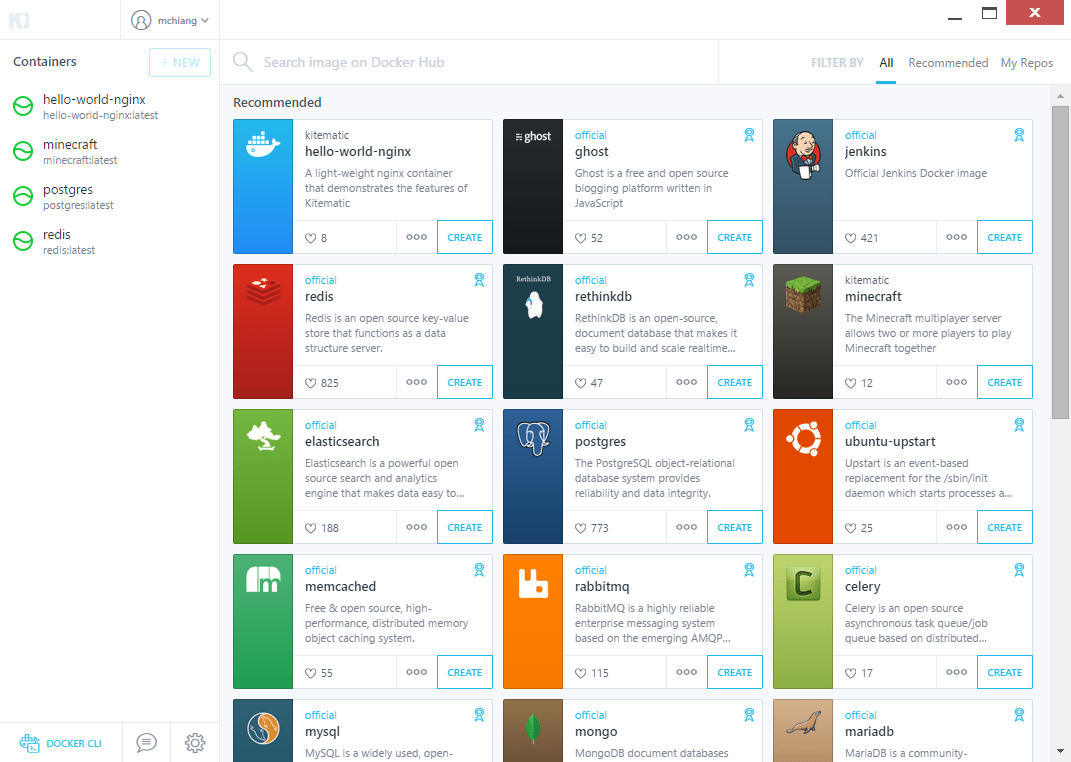
\includegraphics[width=.95\textwidth]{kitematic.png}
\end{frame}

\section{Podsumowanie}

\begin{frame}{Bibliografia i ciekawe źródła}
  
	\begin{thebibliography}{9}
	
		\bibitem{rewak}
		Krzysztof Rewak,
		\textit{Projektowanie i programowanie obiektowe},
		materiały do zajęć laboratoryjnych
	
		\bibitem{rewak2}
		Krzysztof Rewak,
		\textit{Projektowanie i programowanie systemów internetowych I},
		slajdy z wykładów
		
		\bibitem{docker}
		\url{https://www.masterzendframework.com/docker-development-environment/}
	
	\end{thebibliography}

\end{frame}

\appendix

\begin{frame}[standout]
	Pytania?
\end{frame}

\begin{frame}{}

	Kod prezentacji dostępny jest w repozytorium git pod adresem \texttt{https://bitbucket.org/krewak/pwsz-ppsi} \\ \ \\

	\begin{figure}
		\centering
		\href{https://bitbucket.org/krewak/pwsz-ppsi}{
			
\includegraphics[width=.15\textwidth]{../_template/bitbucket.png}
		}
	\end{figure}
	
	Wszystkie informacje dot. kursu dostępne są pod adresem \texttt{http://pwsz.rewak.pl/kursy/4} \\ \ \\

	\begin{figure}
		\centering
		\href{http://pwsz.rewak.pl/kursy/3}{
			
\includegraphics[width=.15\textwidth]{../_template/rewak.png}
		}
	\end{figure}

\end{frame}

\end{document}
